\chapter{Mutasi dan Penganekaragaman Genom}\label{ch:b2:genome-diversification}

Sebarkanlah semiliar bakteri pada sebuah lempeng yang dibubuhi
antibiotik dan, keesokan paginya, segelintir koloni telah tumbuh.
Apakah obatnya mengajari sel-sel itu menahannya, ataukah mereka sudah
kebal sebelum berjumpa dengannya? Pertanyaannya terdengar filosofis
dan diselesaikan sebuah percobaan yang sangat elok pada 1943: sel yang
kebal sudah ada sebelumnya, dihasilkan \omterm{def:b2:genome-diversification:mutation}{mutasi} yang terjadi secara
acak, tanpa menghiraukan kegunaannya. Bab ini membahas sumber
keragaman itu --- kekeliruan penyalinan, kecelakaan kimia, gen yang
melompat, gen yang diperdagangkan antarsel, \omterm{prop:b2:genome-diversification:duplication}{duplikasi gen} dan seluruh
genom --- serta seberapa cepat semuanya berjalan. Seleksi, yang memilah
keragaman itu, adalah pokok \cref{ch:b2:population-genetics}; di sini
pokoknya adalah dari mana bahan mentahnya datang.

\section{Mutasi}

\begin{definition}[Mutasi dan ragamnya]\label{def:b2:genome-diversification:mutation}
\index{mutasi}\index{mutasi titik}\index{pergeseran rangka baca}\index{penataan ulang kromosom}
Sebuah \emph{mutasi} adalah perubahan terwariskan pada urutan
genomnya. \emph{Mutasi titik} mengubah satu atau beberapa basa: sebuah
\emph{substitusi} mengganti satu basa dengan basa lain (sebuah
\emph{transisi} menukar purina dengan purina atau pirimidina dengan
pirimidina, A$\leftrightarrow$G atau C$\leftrightarrow$T; sebuah
\emph{transversi} menukar kelasnya); sebuah \emph{insersi} atau
\emph{delesi} menambah atau membuang basa. Di dalam urutan penyandi,
sebuah substitusi disebut \emph{bisu} kalau kodon barunya menetapkan
asam amino yang sama, \emph{salah arti} kalau ia menetapkan asam amino
lain, \emph{tanpa arti} kalau ia menciptakan sebuah henti; sebuah
insersi atau delesi yang bukan kelipatan tiga menggeser rangka bacanya
(\emph{pergeseran rangka baca}) dan mengacaukan setiap kodon di
hilirnya. \emph{Penataan ulang kromosom} memindahkan ruas besar:
delesi, duplikasi, inversi, translokasi antarkromosom. \emph{Mutasi
genom} mengubah cacah kromosomnya: \emph{aneuploidi} (satu kromosom
berlebih atau berkurang, seperti pada trisomi 21) dan
\emph{\omterm{def:b2:genome-diversification:polyploidy}{poliploidi}} (seluruh perangkat tambahan). Mutasi
pada sel soma hanya diwarisi keturunan sel itu; mutasi pada garis
nutfah diwarisi keturunan organismenya, dan hanya mutasi inilah yang
berarti bagi evolusi.
\end{definition}

\begin{omfigure}
\begin{tikzpicture}[every node/.style={font=\small\ttfamily}]
  \node[anchor=west] at (0,2.4) {ATG GAA TTC CTG AAG TGG TAA};
  \node[anchor=west, font=\scriptsize\rmfamily] at (5.6,2.4) {Met Glu Phe Leu Lys Trp henti --- tipe liar};
  \node[anchor=west] at (0,1.7) {ATG GA\textcolor{omThm}{G} TTC CTG AAG TGG TAA};
  \node[anchor=west, font=\scriptsize\rmfamily] at (5.6,1.7) {Met Glu Phe Leu Lys Trp henti --- bisu};
  \node[anchor=west] at (0,1.0) {ATG G\textcolor{omThm}{T}A TTC CTG AAG TGG TAA};
  \node[anchor=west, font=\scriptsize\rmfamily] at (5.6,1.0) {Met \textcolor{omThm}{Val} Phe Leu Lys Trp henti --- salah arti};
  \node[anchor=west] at (0,0.3) {ATG \textcolor{omThm}{T}AA TTC CTG AAG TGG TAA};
  \node[anchor=west, font=\scriptsize\rmfamily] at (5.6,0.3) {Met \textcolor{omThm}{henti} --- tanpa arti};
  \node[anchor=west] at (0,-0.4) {ATG GA\textcolor{omThm}{C}A TTC CTG AAG TGG TAA};
  \node[anchor=west, font=\scriptsize\rmfamily] at (5.6,-0.4) {Met \textcolor{omThm}{Asp Ile Pro Glu Val} \dots{} --- pergeseran rangka};
\end{tikzpicture}

{\small \omterm{def:b2:genome-diversification:mutation}{Mutasi titik} pada sebuah urutan penyandi pendek (perubahannya
merah). Substitusi bisu mempertahankan proteinnya; substitusi salah
arti mengubah satu residu; substitusi tanpa arti memenggalnya; satu
basa yang disisipkan menggeser rangkanya dan menulis ulang segalanya di
hilirnya.}
\end{omfigure}

\begin{proposition}[Dari mana mutasi datang]\label{prop:b2:genome-diversification:sources}
\index{mutagen}\index{deaminasi}\index{depurinasi}
Ada tiga sumbernya. \emph{Kekeliruan replikasi}: DNA polimerase salah
menaruh sebuah basa kira-kira sekali tiap $10^{5}$; eksonuklease
pengoreksinya membuang sebagian besarnya, dan menyisakan satu tiap
$10^{7}$; perbaikan salah pasang, yang mengikuti garpu replikasinya dan
membetulkan untai baru terhadap untai lama, membawa laju kekeliruan
akhirnya menjadi kira-kira $10^{-9}$ sampai $10^{-10}$ tiap basa tiap
replikasi. \emph{Kimia spontan}: tiap hari, di dalam tiap sel manusia,
sekitar \num{10000} purina lepas dari gulanya
(\emph{depurinasi}) dan seratus sitosina kehilangan gugus aminanya
(\emph{deaminasi}, yang mengubah C menjadi U, yang berpasangan dengan
A); keduanya diperbaiki, tetapi tidak selalu. \emph{Mutagen}: sinar
ultraungu melas timina yang bersebelahan menjadi dimer; radiasi
pengion memutus untai; zat pengalkilasi dan asam nitrit mengubah basa;
zat warna penyisip menyelinap di antara pasangan basa lalu menimbulkan
\omterm{def:b2:genome-diversification:mutation}{pergeseran rangka baca}; radikal oksigen dari
respirasi mengoksidasi guanina. Lajunya tiap basa sangatlah kecil;
dikalikan ukuran genom dan cacah selnya, ia tidak kecil lagi.
\end{proposition}

\begin{theorem}[Mutasi tiap genom dan tiap populasi]\label{thm:b2:genome-diversification:rate}
\index{laju mutasi}
Jika \omterm{thm:b2:genome-diversification:rate}{laju mutasinya} adalah $u$ tiap pasangan basa tiap replikasi dan
genomnya memuat $G$ pasangan basa, tiap replikasi menghasilkan
rata-rata $U = uG$ \omterm{def:b2:genome-diversification:mutation}{mutasi} baru, dan populasi berisi $N$ sel
menghasilkan $UN$ \omterm{def:b2:genome-diversification:mutation}{mutasi} tiap generasi. Bagi \emph{E.~coli}
($u \approx \qty{5e-10}{}$, $G =
\qty{4.6e6}{}$): $U \approx 0.002$, sehingga satu sel dari tiap lima
ratus mengusung sebuah \omterm{def:b2:genome-diversification:mutation}{mutasi} baru --- tetapi biakan berisi $10^{9}$
sel membuat dua juta \omterm{def:b2:genome-diversification:mutation}{mutasi} tiap generasi, dan tiap satu dari
$3G \approx 1.4\times
10^{7}$ perubahan basa tunggal yang mungkin muncul di suatu tempat di
dalamnya tiap beberapa generasi. Bagi manusia
($u \approx \qty{1.2e-8}{}$ tiap generasi, $G = \qty{3.2e9}{}$ tiap
perangkat haploid, dua perangkat): tiap anak mengusung sekitar \num{75} \omterm{def:b2:genome-diversification:mutation}{mutasi}
baru, satu atau dua di antaranya di dalam urutan penyandi.
\end{theorem}
\begin{proof}
Tiap basa disalin secara bebas dengan peluang kekeliruan $u$, sehingga
cacah kekeliruan tiap salinan genomnya adalah jumlah $G$ peristiwa
langka yang saling bebas, dengan purata $uG$ (dan hampiran sebaran
Poisson). $N$ sel membuat $N$ salinan. Angka manusianya mengalikan $u$
dengan $2G$ untuk genom diploidnya; lajunya tiap generasi memang tiap
generasi, bukan tiap replikasi, karena sel nutfah menjalani banyak
replikasi antara pembuahan dan pembuahan berikutnya.
\end{proof}

\begin{theorem}[Mutan di dalam biakan yang tumbuh]\label{thm:b2:genome-diversification:luria}
\index{percobaan Luria--Delbrück}\index{uji fluktuasi}
Sebuah biakan yang tumbuh dari $N_0$ menjadi $N$ sel, yang di dalamnya
sebuah \omterm{def:b2:genome-diversification:mutation}{mutasi} tertentu terjadi dengan peluang $m$ pada tiap pembelahan
sel, pada akhirnya memuat purata cacah \emph{peristiwa} \omterm{def:b2:genome-diversification:mutation}{mutasi}
$m(N - N_0)$, dan purata cacah \emph{sel} mutan
\[
\langle M\rangle = m\,N\,\ln\frac{N}{N_0},
\]
yang lebih besar daripada cacah peristiwanya karena \omterm{def:b2:genome-diversification:mutation}{mutasi} yang dini
mendirikan sebuah klon. Cacah sel mutannya berbeda-beda luar biasa dari
biakan ke biakan (peristiwa dini yang langka memberi ``jekpot''),
sedangkan kalau \omterm{def:b2:genome-diversification:mutation}{mutasinya} diimbas pada saat pelempengan, cacahnya akan
mengikuti hukum Poisson dengan ragam sama dengan puratanya. Bagian
biakan yang sama sekali tidak bermutan adalah $p_0 = e^{-m(N - N_0)}$,
yang memberikan $m$ secara langsung.
\end{theorem}
\begin{proof}
Pertumbuhan dari $n$ menjadi $n + \mathrm{d}n$ sel memakan
$\mathrm{d}n$ pembelahan, masing-masing sebuah peluang bagi \omterm{def:b2:genome-diversification:mutation}{mutasinya},
sehingga $m\,\mathrm{d}n$ peristiwa terjadi pada selang itu; dijumlahkan,
seluruhnya $m(N - N_0)$ peristiwa. Sebuah \omterm{def:b2:genome-diversification:mutation}{mutasi} yang terjadi ketika
biakannya berisi $n$ sel mendirikan sebuah klon yang tumbuh seirama
dengan biakannya dan berjumlah $N/n$ sel pada akhirnya; maka harapan
cacah sel mutannya adalah
$\int_{N_0}^{N} m\,(N/n)\,\mathrm{d}n = mN\ln(N/N_0)$. Peristiwanya
langka dan saling bebas, sehingga cacahnya berdistribusi Poisson dengan
purata $m(N - N_0)$, dan peluang tidak ada satu pun adalah
$e^{-m(N - N_0)}$.
\end{proof}
\begin{proof}[Bukti eksperimental]
Luria dan Delbrück (1943) menumbuhkan dua puluh biakan kecil
\emph{E.~coli} masing-masing dari beberapa sel, dan sejajar dengan itu
mengambil dua puluh contoh dari satu biakan besar; mereka melempengkan
keempat puluhnya dengan bakteriofag yang membunuh setiap sel yang peka
lalu mencacah koloni yang kebal. Contoh dari biakan tunggalnya memberi
cacah yang dekat dengan puratanya, seperti diramalkan hukum Poisson;
biakan yang saling bebas memberi cacah 0, 0, 1, 0, 3, 0, 107, 0,
5\dots{} --- ragam yang berlipat-lipat puratanya. \omterm{def:b2:genome-diversification:mutation}{Mutasi} menuju
kekebalan telah terjadi pada waktu yang acak \emph{sebelum} selnya
berjumpa dengan fagnya, dan yang dini menghasilkan jekpot. Lederberg
dan Lederberg (1952) menegaskannya tanpa pernah memaparkan sel
terseleksinya kepada zatnya: dengan menekankan bantalan beledu pada
sebuah lempeng lalu mencapkan salinannya, mereka mendapati koloni yang
kebal pada kedudukan yang sama di tiap replikanya, lalu mengisolasinya
dari lempeng induk yang tak pernah diperlakukan.
\end{proof}

\begin{omfigure}
\begin{tikzpicture}[every node/.style={font=\scriptsize}, level distance=0.55cm, sibling distance=0.5cm, edge from parent/.style={draw, gray}]
  \begin{scope}
    \node[circle, fill=omDef!40, inner sep=1.5pt] (r) at (0,0) {}
      child { node[circle, fill=omDef!40, inner sep=1.5pt] {}
        child { node[circle, fill=omDef!40, inner sep=1.5pt] {} child { node[circle, fill=omDef!40, inner sep=1.5pt] {} } child { node[circle, fill=omDef!40, inner sep=1.5pt] {} } }
        child { node[circle, fill=omDef!40, inner sep=1.5pt] {} child { node[circle, fill=omDef!40, inner sep=1.5pt] {} } child { node[circle, fill=omThm, inner sep=1.5pt] {} } } }
      child { node[circle, fill=omDef!40, inner sep=1.5pt] {}
        child { node[circle, fill=omDef!40, inner sep=1.5pt] {} child { node[circle, fill=omDef!40, inner sep=1.5pt] {} } child { node[circle, fill=omDef!40, inner sep=1.5pt] {} } }
        child { node[circle, fill=omDef!40, inner sep=1.5pt] {} child { node[circle, fill=omDef!40, inner sep=1.5pt] {} } child { node[circle, fill=omDef!40, inner sep=1.5pt] {} } } };
    \node[align=center] at (0,-2.4) {mutasi lambat:\\satu sel mutan};
  \end{scope}
  \begin{scope}[xshift=5cm]
    \node[circle, fill=omDef!40, inner sep=1.5pt] at (0,0) {}
      child { node[circle, fill=omThm, inner sep=1.5pt] {}
        child { node[circle, fill=omThm, inner sep=1.5pt] {} child { node[circle, fill=omThm, inner sep=1.5pt] {} } child { node[circle, fill=omThm, inner sep=1.5pt] {} } }
        child { node[circle, fill=omThm, inner sep=1.5pt] {} child { node[circle, fill=omThm, inner sep=1.5pt] {} } child { node[circle, fill=omThm, inner sep=1.5pt] {} } } }
      child { node[circle, fill=omDef!40, inner sep=1.5pt] {}
        child { node[circle, fill=omDef!40, inner sep=1.5pt] {} child { node[circle, fill=omDef!40, inner sep=1.5pt] {} } child { node[circle, fill=omDef!40, inner sep=1.5pt] {} } }
        child { node[circle, fill=omDef!40, inner sep=1.5pt] {} child { node[circle, fill=omDef!40, inner sep=1.5pt] {} } child { node[circle, fill=omDef!40, inner sep=1.5pt] {} } } };
    \node[align=center] at (0,-2.4) {mutasi dini:\\jekpot berisi empat};
  \end{scope}
  \begin{scope}[xshift=10cm]
    \node[circle, fill=omDef!40, inner sep=1.5pt] at (0,0) {}
      child { node[circle, fill=omDef!40, inner sep=1.5pt] {}
        child { node[circle, fill=omDef!40, inner sep=1.5pt] {} child { node[circle, fill=omDef!40, inner sep=1.5pt] {} } child { node[circle, fill=omThm, inner sep=1.5pt] {} } }
        child { node[circle, fill=omDef!40, inner sep=1.5pt] {} child { node[circle, fill=omDef!40, inner sep=1.5pt] {} } child { node[circle, fill=omDef!40, inner sep=1.5pt] {} } } }
      child { node[circle, fill=omDef!40, inner sep=1.5pt] {}
        child { node[circle, fill=omDef!40, inner sep=1.5pt] {} child { node[circle, fill=omThm, inner sep=1.5pt] {} } child { node[circle, fill=omDef!40, inner sep=1.5pt] {} } }
        child { node[circle, fill=omDef!40, inner sep=1.5pt] {} child { node[circle, fill=omDef!40, inner sep=1.5pt] {} } child { node[circle, fill=omDef!40, inner sep=1.5pt] {} } } };
    \node[align=center] at (0,-2.4) {kalau diimbas saat pelempengan:\\taburan Poisson};
  \end{scope}
\end{tikzpicture}

{\small \omterm{thm:b2:genome-diversification:luria}{Uji fluktuasi}. Kalau \omterm{def:b2:genome-diversification:mutation}{mutasi} (merah) terjadi secara acak
selama pertumbuhannya, cacah mutannya bergantung pada \emph{kapan}
\omterm{def:b2:genome-diversification:mutation}{mutasinya} terjadi, dan biakan yang saling bebas berbeda liar; kalau zat
penyeleksinya mengimbasnya pada saat pelempengan, tiap biakan akan
menunjukkan cacah kecil yang serupa.}
\end{omfigure}

\begin{omfigure}
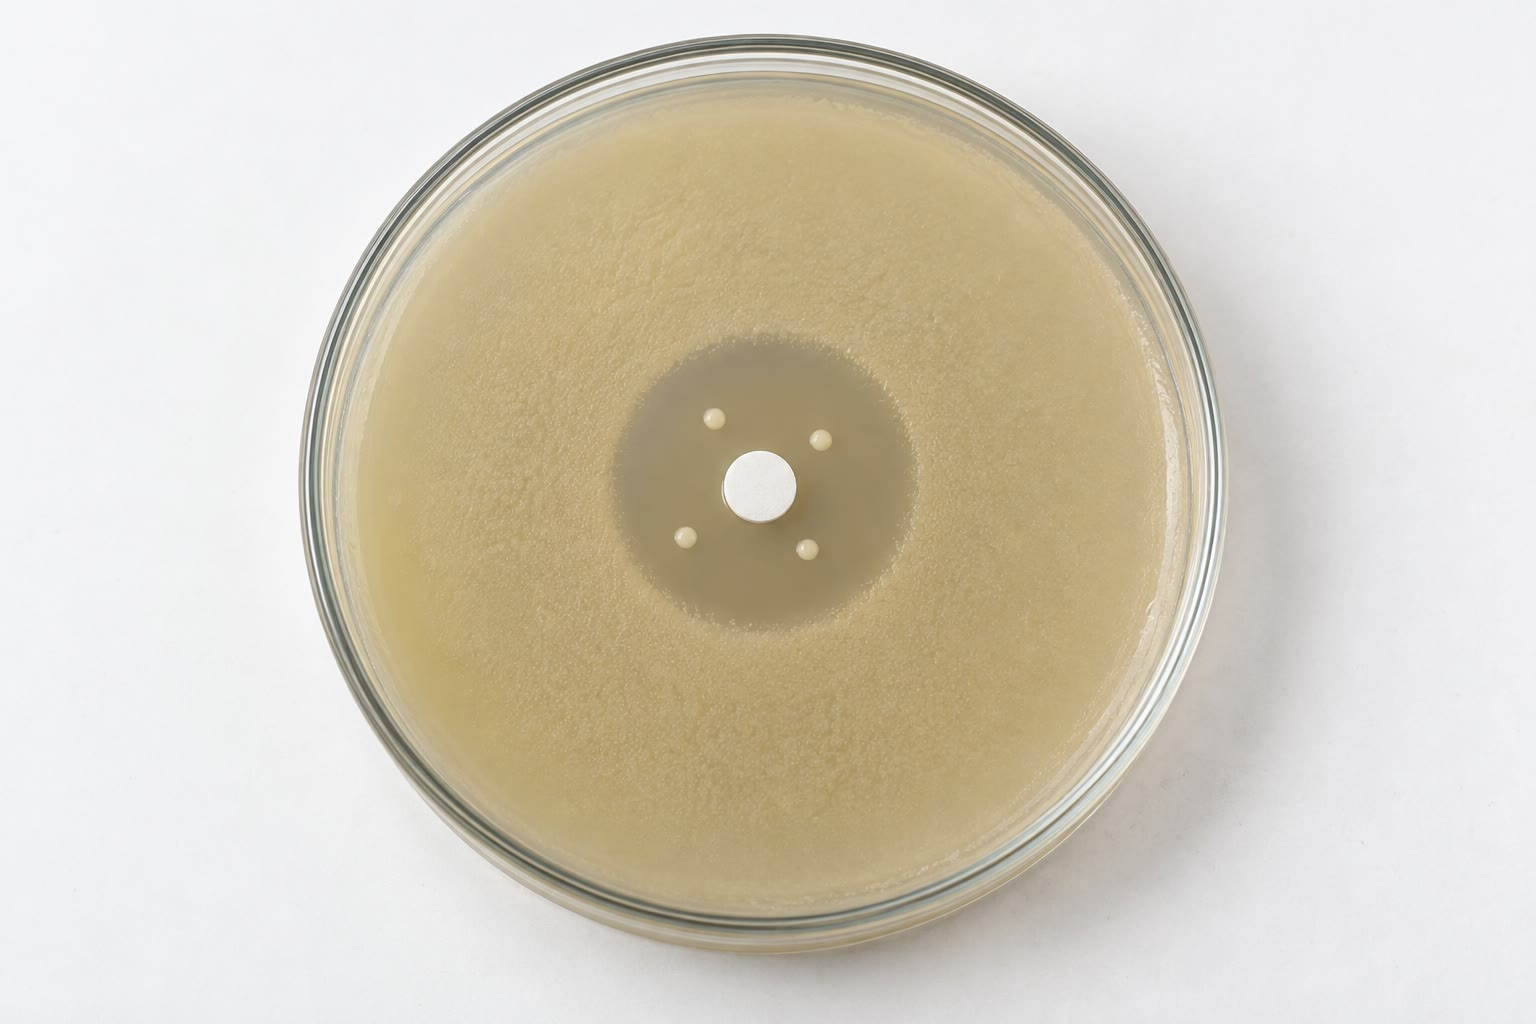
\includegraphics[width=0.5\linewidth]{images/book4/ai/b4-03-luria-plate.jpg}

{\small Sebuah cakram antibiotik pada hamparan bakteri: daerah
beningnya adalah tempat obat yang berdifusi dari cakramnya telah
membunuh sel yang peka, dan koloni di dalamnya tumbuh dari mutan kebal
yang sudah ada sebelum cakramnya diletakkan.}
\end{omfigure}

\begin{proposition}[Perbaikan dan batasnya]\label{prop:b2:genome-diversification:repair}
\index{perbaikan DNA}
Sebuah sel membetulkan sebagian besar kerusakannya sebelum kerusakan
itu menjadi \omterm{def:b2:genome-diversification:mutation}{mutasi}. \emph{Perbaikan salah pasang} membuang basa yang
keliru dari untai yang baru dibuat. \emph{Perbaikan eksisi basa}
memotong satu basa yang rusak (sebuah urasil, sebuah guanina
teroksidasi) lalu mengisi celahnya; inilah sebabnya DNA memakai timina
alih-alih urasil: sebuah urasil di dalam DNA hanya mungkin sitosina
yang terdeaminasi, dan dikenali sebagai asing. \emph{Perbaikan eksisi
nukleotida} membuang seruas selusin basa di sekeliling lesi besar
seperti dimer timina; orang yang tidak memilikinya (xeroderma
pigmentosum) terkena kanker kulit dari sinar matahari biasa.
\emph{Perbaikan rekombinasional} membangun kembali kromosom yang putus
dari salinan saudarinya. Yang lolos dari perbaikan, atau yang
diperbaiki secara keliru, menjadi \omterm{def:b2:genome-diversification:mutation}{mutasi} --- dan sel yang telah
kehilangan sebuah sistem perbaikan (seorang \emph{mutator}) bermutasi
seratus kali lebih cepat, yang merupakan keuntungan jangka pendek di
bawah tekanan dan beban jangka panjang. Mekanisme perbaikannya dibahas
mendalam dalam jilid Tahun ke-3.
\end{proposition}

\section{Gen yang berpindah}

\begin{definition}[Unsur dapat berpindah]\label{def:b2:genome-diversification:transposon}
\index{transposon}\index{retrotransposon}
Sebuah \emph{unsur dapat berpindah} adalah ruas DNA yang dapat
berpindah ke kedudukan baru di dalam genomnya. \emph{Transposon DNA}
menyandikan sebuah \emph{transposase} yang memotong unsurnya keluar
lalu menempelkannya di tempat lain (atau menyalinnya ke sana); urutan
sisipan bakteri adalah yang paling sederhana (sebuah gen transposase di
antara dua ulangan terbalik), dan transposon majemuk mengusung gen
tambahan --- kerap kekebalan antibiotik --- di antara dua urutan
sisipan. \emph{Retrotransposon} berpindah lewat jalan salin-dan-tempel
melalui perantara RNA, yang disalin kembali menjadi DNA oleh sebuah
transkriptase balik; mereka tidak pernah meninggalkan tapak lamanya
sehingga menimbun. Sebuah unsur yang mendarat di dalam sebuah gen
merusaknya; mendarat di dekat sebuah gen, ia dapat mengubah
pengungkapannya; dua salinan dalam satu kromosom menyediakan tapak bagi
\omterm{prop:b2:genome-diversification:duplication}{pindah silang tak setara}. Transposon dan peninggalannya menyusun
separuh genom manusia dan delapan puluh persen genom jagung; sebagian
besarnya kini tak bergerak lagi.
\end{definition}
\begin{proof}[Bukti eksperimental]
McClintock (1940-an--1950-an) menelaah biji jagung yang pigmen ungunya
hilang pada sebagian sel dan pulih pada sel yang lain, sehingga
bijinya berbintik-bintik. Ia menunjukkan lewat pemuliaan dan lewat
pengamatan kromosom bahwa ketakmantapan itu disebabkan sebuah unsur
(\emph{Disosiasi}) yang mematahkan kromosom di tempatnya duduk lalu
berpindah antarkedudukan di bawah kendali unsur kedua
(\emph{Aktivator}), dan bahwa sebuah gen dibungkam ketika unsurnya
duduk di dalamnya lalu diaktifkan kembali ketika unsurnya pergi. Gen,
simpulnya, dapat berganti kedudukan; gagasannya baru diterima dua
puluh tahun kemudian, ketika urutan sisipan bakteri ditemukan, dan
membuatnya meraih Hadiah Nobel pada 1983.
\end{proof}

\begin{omfigure}
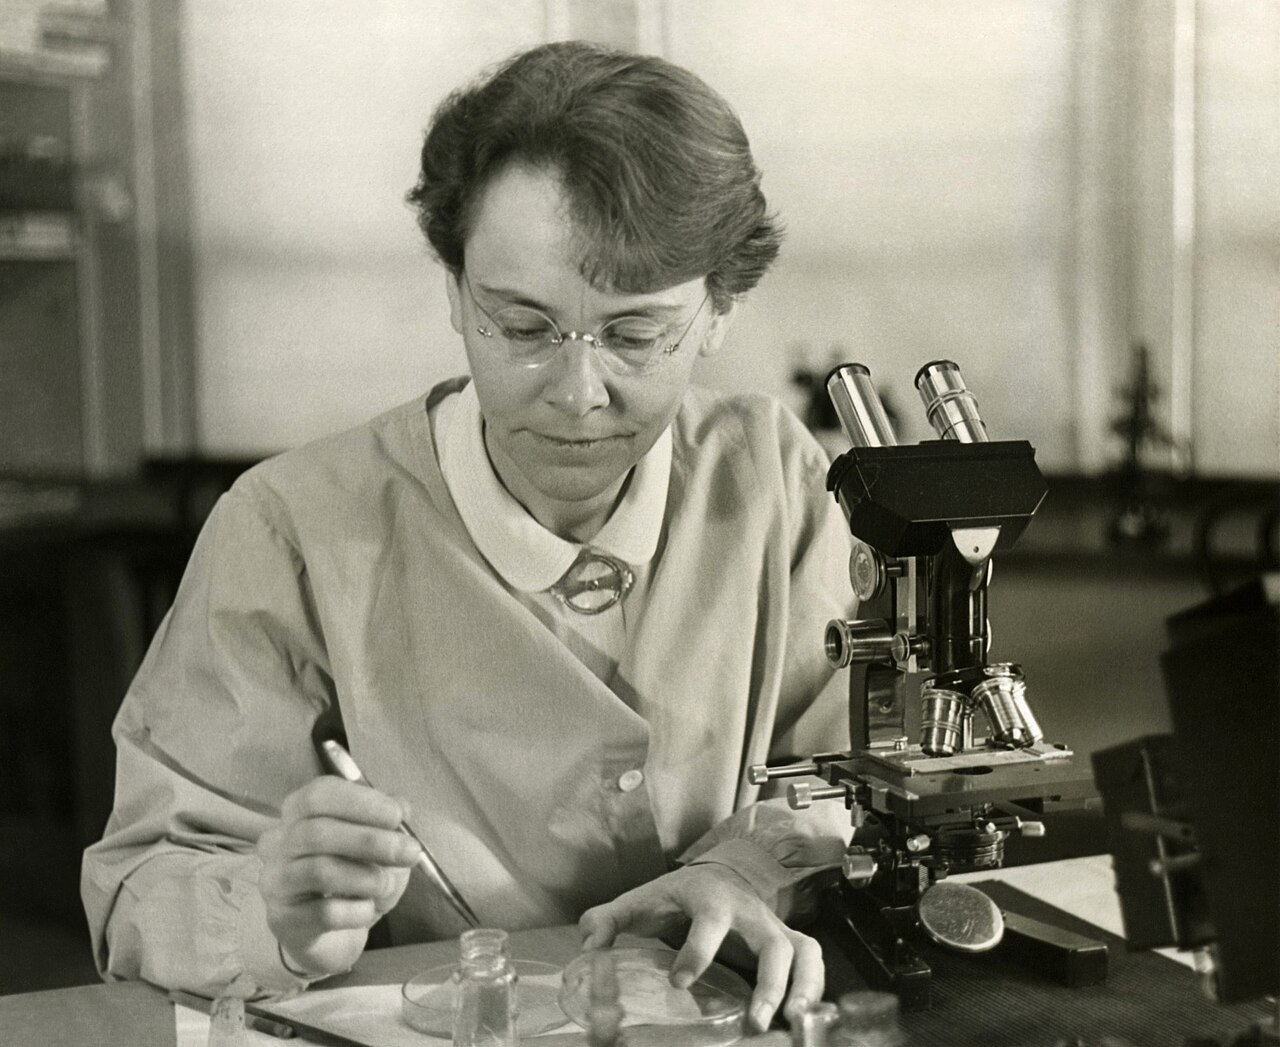
\includegraphics[width=0.4\linewidth]{images/book4/mcclintock.jpg}\hspace{0.04\linewidth}
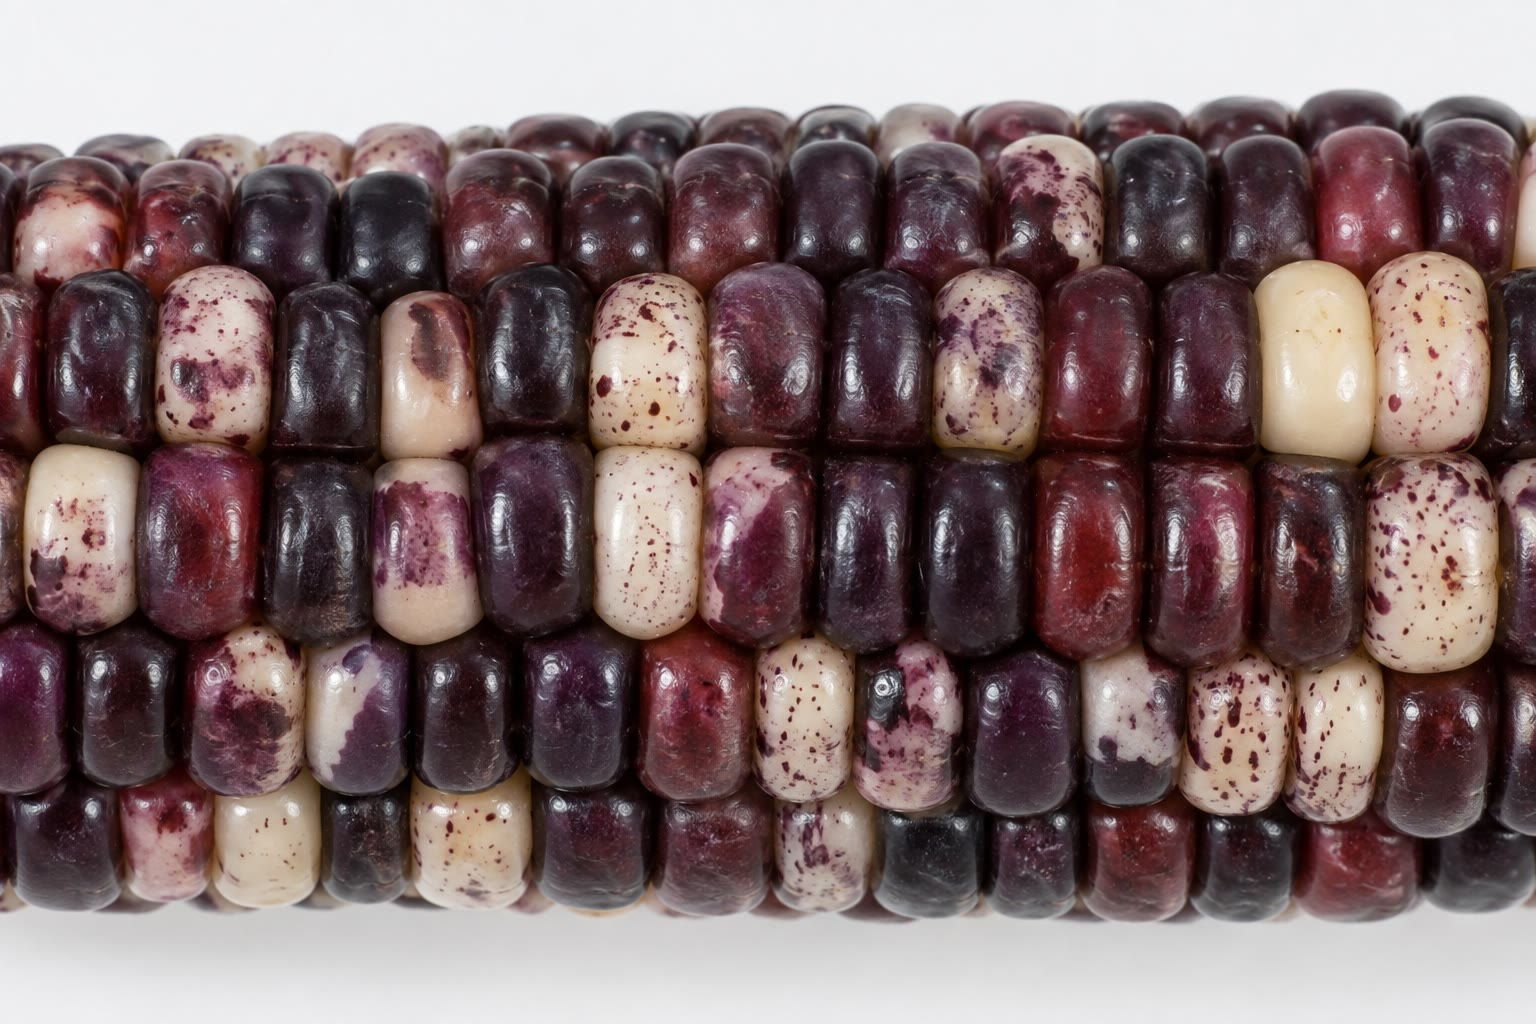
\includegraphics[width=0.5\linewidth]{images/book4/ai/b4-03-maize-kernels.jpg}

{\small Barbara McClintock, dan biji jagung yang menuntunnya kepada
unsur dapat berpindah: sebuah gen pigmen ungu yang dimatikan unsur
yang menyisip lalu dinyalakan kembali, sel demi sel, ketika unsurnya
melompat keluar, dan meninggalkan bintik serta juring.}
\end{omfigure}

\begin{omfigure}
\begin{tikzpicture}[every node/.style={font=\scriptsize}]
  % cut and paste
  \begin{scope}
    \draw[very thick, gray] (0,1.2) -- (4.5,1.2);
    \fill[omThm!70] (0.8,1.05) rectangle (1.8,1.35); \node[white, font=\tiny] at (1.3,1.2) {Tn};
    \draw[very thick, gray] (0,0) -- (4.5,0);
    \fill[omThm!70] (2.8,-0.15) rectangle (3.8,0.15); \node[white, font=\tiny] at (3.3,0) {Tn};
    \draw[->, thick, omThm] (1.3,1.0) .. controls (1.3,0.5) and (3.3,0.7) .. (3.3,0.2);
    \draw[dashed, gray] (0.8,1.2) -- (1.8,1.2);
    \node[align=center] at (2.25,-0.6) {potong dan tempel (transposon DNA):\\unsurnya meninggalkan tapak lamanya};
  \end{scope}
  % copy and paste
  \begin{scope}[xshift=7.5cm]
    \draw[very thick, gray] (0,1.2) -- (4.5,1.2);
    \fill[omProp!80] (0.8,1.05) rectangle (1.8,1.35); \node[white, font=\tiny] at (1.3,1.2) {RT};
    \draw[very thick, gray] (0,0) -- (4.5,0);
    \fill[omProp!80] (2.8,-0.15) rectangle (3.8,0.15); \node[white, font=\tiny] at (3.3,0) {RT};
    \draw[->, thick, omProp] (1.3,1.0) .. controls (1.3,0.5) and (3.3,0.7) .. (3.3,0.2);
    \node[omProp, anchor=west, align=left] at (3.6,0.75) {salinan RNA,\\ditranskripsi balik};
    \node[align=center] at (2.25,-0.6) {salin dan tempel (retrotransposon):\\salinan lamanya tinggal, cacahnya tumbuh};
  \end{scope}
\end{tikzpicture}

{\small Dua cara berpindah. Sebuah \omterm{def:b2:genome-diversification:transposon}{transposon} DNA dieksisi lalu
disisipkan kembali; sebuah \omterm{def:b2:genome-diversification:transposon}{retrotransposon} ditranskripsi, disalin
kembali menjadi DNA, lalu disisipkan di tempat lain, sehingga
salinannya menimbun.}
\end{omfigure}

\begin{definition}[Pemindahan gen mendatar]\label{def:b2:genome-diversification:hgt}
\index{pemindahan gen mendatar}\index{transformasi}\index{konjugasi!bakteri}\index{transduksi}
\omterm{def:b2:unicellular-diversity:prokaryote}{Prokariot} memperoleh gen dari sel yang bukan induknya lewat tiga jalan.
\emph{Transformasi}: sebuah sel menyerap DNA telanjang dari
sekelilingnya (yang dilepaskan sel yang mati) lalu merekombinasikannya
ke dalam kromosomnya; sebagian spesies berkompeten secara alami, dan
inilah jalan pneumokokus bertukar gen kapsul. \emph{Konjugasi}:
seorang pemberi yang mengusung \omterm{def:b2:unicellular-diversity:prokaryote}{plasmid} konjugatif (faktor F
\emph{E.~coli}) membangun sebuah pilus, menarik seorang penerima
mendekat, lalu melewatkan satu untai tunggal \omterm{def:b2:unicellular-diversity:prokaryote}{plasmidnya} melalui sebuah
liang sembari mereplikasinya dengan lingkaran bergulir; kalau
\omterm{def:b2:unicellular-diversity:prokaryote}{plasmidnya} telah bersatu ke dalam kromosomnya (galur Hfr), gen
kromosomnya dipindahkan berurutan di belakangnya, dan waktu masuknya
masing-masing memetakan kromosomnya. \emph{Transduksi}: sebuah
bakteriofag secara keliru mengemas sekeping DNA inangnya lalu
menyuntikkannya ke dalam sel berikutnya yang dijangkitinya. Bersama-sama
jalan ini memindahkan gen kekebalan antarspesies di dalam rumah sakit
dalam hitungan tahun, dan telah memindahkan gen metabolik menyeberangi
seluruh pohon bakteri sepanjang waktu geologi, sehingga silsilah
sebuah \omterm{def:b2:unicellular-diversity:prokaryote}{prokariot} adalah sebuah jaring sama banyaknya dengan sebuah
pohon (\cref{ch:b2:phylogenetic-trees}).
\end{definition}
\begin{proof}[Bukti eksperimental]
Lederberg dan Tatum (1946) mencampur dua galur \emph{E.~coli}, yang
masing-masing tak sanggup membuat dua hara yang berbeda, lalu
melempengkan campurannya pada medium minimal yang tak satu pun dapat
tumbuh sendirian di atasnya: koloni bermunculan, kira-kira satu tiap
sepuluh juta sel, yang sanggup membuat keempatnya --- rekombinan.
Davis (1950) mengulanginya dengan kedua galurnya dipisahkan sebuah
saringan yang melewatkan molekul tetapi tidak sel: tidak ada
rekombinan, sehingga sentuhan memang dibutuhkan. Hayes lalu menunjukkan
pemindahannya searah, dari seorang pemberi kepada seorang penerima, dan
Wollman serta Jacob (1956) memutus perkawinannya dengan pengaduk pada
selang waktu tertentu lalu mendapati gen pemberinya memasuki penerimanya
menurut urutan tetap, satu demi satu, selama kira-kira seratus menit.
\end{proof}

\begin{omfigure}
\begin{minipage}[b]{0.56\linewidth}\centering
\begin{tikzpicture}[every node/.style={font=\scriptsize}]
  % donor
  \draw[thick, fill=omDef!8] (0,0) ellipse (1.5 and 0.75);
  \draw[thick, omDef] (0.2,0) circle (0.45);
  \draw[thick, omThm] (-0.9,0.1) circle (0.22);
  \node[anchor=south] at (0,1.25) {pemberi $F^+$};
  \draw[omThm] (-0.9,-0.12) -- (-1.1,-1.0) node[below] {plasmid F};
  \draw[omDef] (0.4,-0.4) -- (0.6,-1.0) node[below] {kromosom};
  % recipient
  \draw[thick, fill=omDef!8] (5,0) ellipse (1.5 and 0.75);
  \draw[thick, omDef] (5.2,0) circle (0.45);
  \node[anchor=south] at (5,1.25) {penerima $F^-$};
  % pilus
  \draw[very thick, omThm] (1.5,0) -- (3.5,0);
  \node[omThm, below] at (2.5,-0.05) {pilus};
  % single strand transferred
  \draw[->, thick, omThm, dashed] (-0.7,0.15) .. controls (1.0,0.7) and (3.0,0.7) .. (4.1,0.4);
  \node[omThm, anchor=south] at (2.5,0.7) {satu untai disalin dengan lingkaran bergulir};
  \draw[thick, omThm, dashed] (4.1,0.2) circle (0.2);
\end{tikzpicture}
\end{minipage}\hfill
\begin{minipage}[b]{0.42\linewidth}\centering
\begin{tikzpicture}
\begin{axis}[
  width=\linewidth, height=4.6cm,
  axis x line=bottom, axis y line=left,
  xmin=0, xmax=40, ymin=0, ymax=1.1,
  xlabel={menit sebelum pengadukan}, ylabel={rekombinan (relatif)},
  xlabel style={font=\scriptsize, at={(axis description cs:0.5,-0.18)}, anchor=north},
  ylabel style={font=\scriptsize},
  tick label style={font=\scriptsize}, xtick={0,10,20,30,40}, ytick={0,0.5,1},
  legend style={font=\scriptsize, at={(0.97,0.08)}, anchor=south east, draw=none},
  clip=false,
]
\addplot[very thick, omDef, domain=8:40, samples=40] {1-exp(-(x-8)/5)};
\addlegendentry{\emph{thr}, masuk pada \qty{8}{min}}
\addplot[very thick, omProp, domain=17:40, samples=40] {1-exp(-(x-17)/5)};
\addlegendentry{\emph{lac}, \qty{17}{min}}
\addplot[very thick, omThm, domain=25:40, samples=40] {1-exp(-(x-25)/5)};
\addlegendentry{\emph{gal}, \qty{25}{min}}
\end{axis}
\end{tikzpicture}
\end{minipage}

{\small Kiri: konjugasi --- pemberinya melewatkan satu untai \omterm{def:b2:unicellular-diversity:prokaryote}{plasmid}
F-nya melalui sambungan pilusnya sembari menyalinnya. Kanan: percobaan
perkawinan terputus dengan seorang pemberi Hfr: tiap gen kromosomnya
mulai muncul di antara rekombinannya pada waktu yang khas, dan waktu
itu memetakan kromosomnya dalam satuan menit.}
\end{omfigure}

\begin{omfigure}
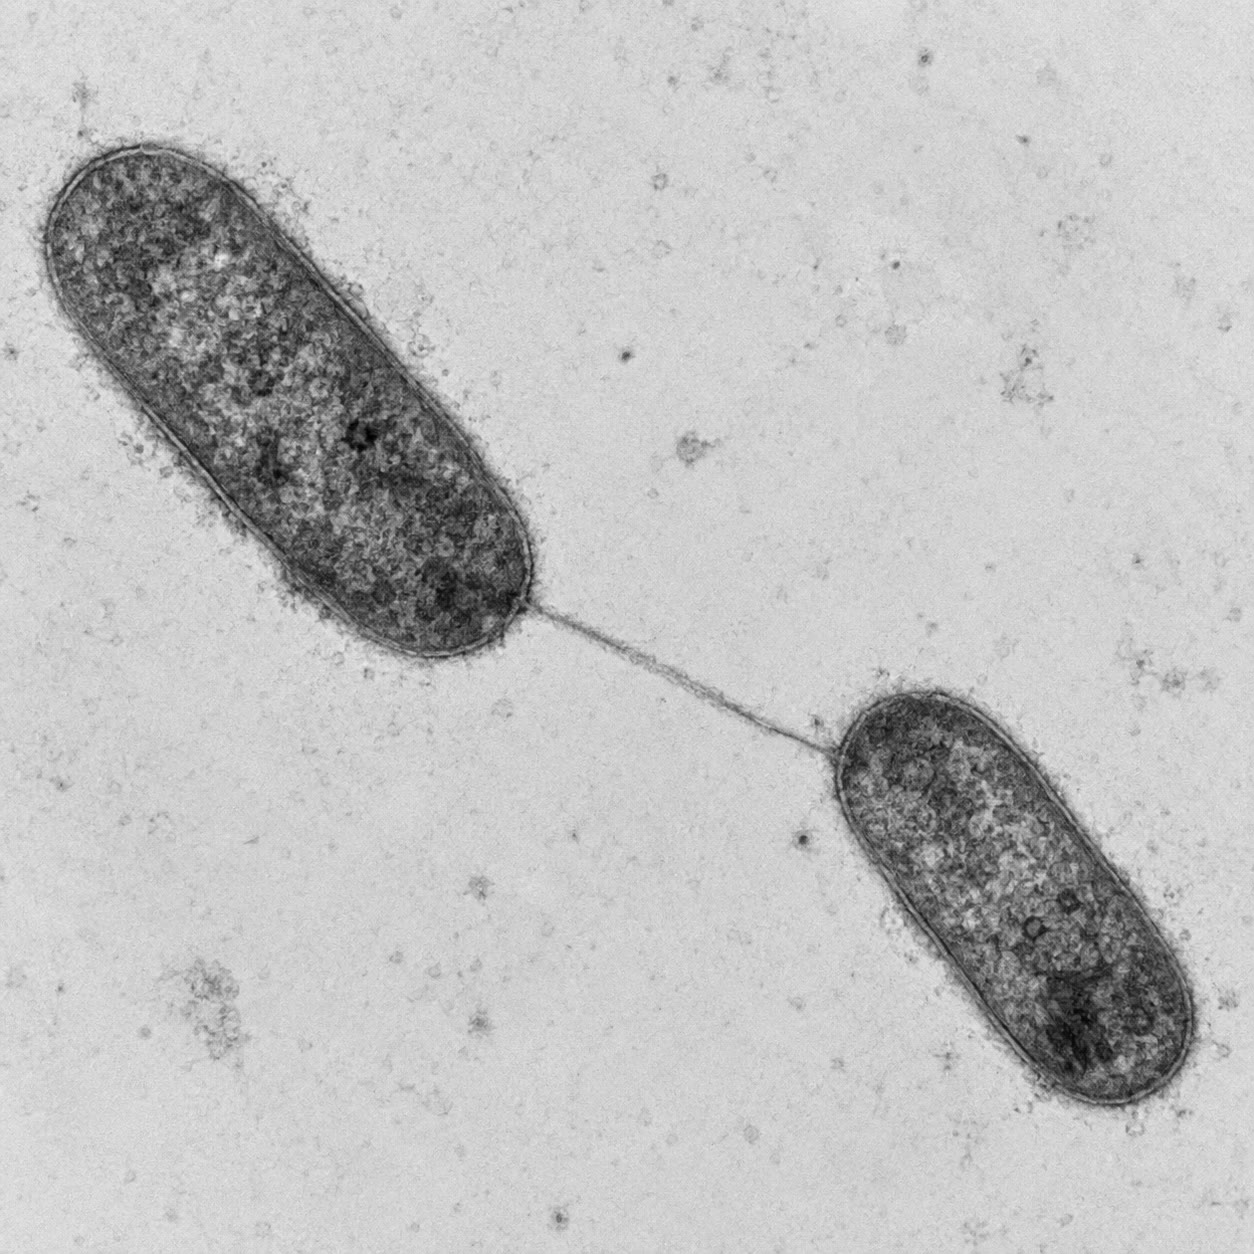
\includegraphics[width=0.42\linewidth]{images/book4/ai/b4-03-conjugation-tem.jpg}

{\small Dua bakteri yang tersambung oleh sebuah pilus konjugatif,
dilihat dengan mikroskopi elektron transmisi: jembatan tempat
\omterm{def:b2:unicellular-diversity:prokaryote}{plasmidnya} lewat.}
\end{omfigure}

\begin{example}[Kekebalan yang berpindah]\label{ex:b2:genome-diversification:resistance}
Sebuah gen kekebalan lazimnya muncul sekali saja, lewat \omterm{def:b2:genome-diversification:mutation}{mutasi} atau
dari bakteri tanah yang membuat antibiotiknya, lalu mengembara: dari
sebuah kromosom ke sebuah \omterm{def:b2:genome-diversification:transposon}{transposon}, dari \omterm{def:b2:genome-diversification:transposon}{transposon} ke sebuah
\omterm{def:b2:unicellular-diversity:prokaryote}{plasmid} konjugatif, dari \omterm{def:b2:unicellular-diversity:prokaryote}{plasmid} menyeberangi spesies lewat konjugasi
dan menyeberangi galur lewat \omterm{def:b2:genome-diversification:hgt}{transduksi}, lalu kembali ke sebuah
kromosom lewat \omterm{def:b2:genome-diversification:hgt}{transformasi}. \omterm{def:b2:unicellular-diversity:prokaryote}{Plasmid} yang mengusung lima atau enam
kekebalan sekaligus (yang dirakit di dalam \emph{integron}, yang
menangkap kaset gen) ditemukan di Jepang pada 1950-an, beberapa tahun
sesudah obatnya mulai dipakai; gen karbapenemase NDM-1, yang pertama
kali terlihat pada 2008, mencapai setiap benua dalam tiga tahun di atas
sebuah \omterm{def:b2:unicellular-diversity:prokaryote}{plasmid}. Evolusi kekebalan sebagian besar bukanlah evolusi gen
baru melainkan perpindahan gen lama.
\end{example}

\section{Duplikasi: gen dan genom}

\begin{proposition}[Duplikasi gen dan keluarga gen]\label{prop:b2:genome-diversification:duplication}
\index{duplikasi gen}\index{keluarga gen}%
\index{pindah silang tak setara}
Ketika dua urutan yang serupa duduk berderet pada sebuah kromosom,
homolognya dapat berpasangan di luar jajarannya pada meiosis lalu
berpindah silang secara tak setara, sehingga satu hasilnya mengusung
tiga salinan dan yang lain satu salinan. Gen yang terduplikasi menjadi
berlebih: satu salinan dapat memegang pekerjaan lamanya sementara yang
lain menimbun \omterm{def:b2:genome-diversification:mutation}{mutasi} dengan bebas --- biasanya meluruh
menjadi sebuah \emph{pseudogen}, sesekali memperoleh fungsi baru
(\emph{neofungsionalisasi}) atau sebagian fungsi lamanya
(\emph{subfungsionalisasi}). Diulangi selama ratusan juta
tahun, hal ini membangun \emph{\omterm{prop:b2:genome-diversification:duplication}{keluarga gen}}: globin (satu gen moyang
menjadi mioglobin, gugusan $\alpha$ dan gugusan $\beta$, dengan anggota
embrionik, janin, dan dewasa yang diungkapkan bergiliran), reseptor
pembau (seribu gen pada seekor mencit), gen homeobox, kristalin lensa.
Sebagian besar gen sebuah genom tergolong ke dalam sebuah keluarga, dan
duplikasi adalah sumber utama gen baru.
\end{proposition}
\begin{proof}[Bukti eksperimental]
Gugusan $\beta$-globin manusia pada kromosom 11 memuat lima gen
berfungsi ($\varepsilon$, $^{G}\gamma$, $^{A}\gamma$,
$\delta$, $\beta$) dan sebuah pseudogen, dalam urutan penyalaannya
selama perkembangan, semuanya berstruktur ekson--intron yang sama, dan
urutannya makin mirip makin baru pemisahannya; gugusan $\alpha$ pada
kromosom 16 memiliki arsitektur yang sama. Delesi satu atau beberapa
gen $\alpha$, yang dihasilkan \omterm{prop:b2:genome-diversification:duplication}{pindah silang tak setara} antara salinan
yang nyaris serupa, sering terjadi dan menyebabkan talasemia $\alpha$;
hasil timbal baliknya, sebuah kromosom dengan tiga gen $\alpha$,
ditemukan pada populasi yang sama.
\end{proof}

\begin{omfigure}
\begin{tikzpicture}[every node/.style={font=\scriptsize}]
  % unequal crossing over
  \begin{scope}
    \draw[very thick, gray] (0,1.2) -- (5,1.2);
    \fill[omDef!70] (1.0,1.05) rectangle (2.0,1.35); \fill[omDef!70] (2.4,1.05) rectangle (3.4,1.35);
    \draw[very thick, gray] (0,0) -- (5,0);
    \fill[omDef!70] (1.0,-0.15) rectangle (2.0,0.15); \fill[omDef!70] (2.4,-0.15) rectangle (3.4,0.15);
    \node[above] at (1.5,1.35) {A}; \node[above] at (2.9,1.35) {A$'$};
    \draw[very thick, omThm] (2.9,1.05) -- (1.5,0.15);
    \node[align=center] at (2.5,-0.6) {homolog yang salah pasang\\berpindah silang tak setara};
    \draw[->, thick, gray] (5.3,0.6) -- (6.1,0.6);
    % products
    \draw[very thick, gray] (6.5,1.2) -- (11.5,1.2);
    \fill[omDef!70] (7.5,1.05) rectangle (8.5,1.35); \fill[omDef!70] (8.9,1.05) rectangle (9.9,1.35); \fill[omDef!70] (10.3,1.05) rectangle (11.3,1.35);
    \node[above] at (9.4,1.35) {tiga salinan};
    \draw[very thick, gray] (6.5,0) -- (11.5,0);
    \fill[omDef!70] (7.5,-0.15) rectangle (8.5,0.15);
    \node[above] at (8.0,0.15) {satu salinan};
  \end{scope}
  % globin family tree
  \begin{scope}[yshift=-3.6cm]
    \draw[thick] (2,2.2) -- (2,1.7);
    \draw[thick] (0.5,1.7) -- (3.5,1.7);
    \draw[thick] (0.5,1.7) -- (0.5,0.4); \node[below] at (0.5,0.4) {mioglobin};
    \draw[thick] (3.5,1.7) -- (3.5,1.2);
    \draw[thick] (2.3,1.2) -- (4.7,1.2);
    \draw[thick] (2.3,1.2) -- (2.3,0.4); \node[below] at (2.3,0.4) {keluarga $\alpha$};
    \draw[thick] (4.7,1.2) -- (4.7,0.9);
    \draw[thick] (3.6,0.9) -- (5.8,0.9);
    \draw[thick] (3.6,0.9) -- (3.6,0.4); \node[below] at (3.6,0.4) {$\varepsilon,\gamma$};
    \draw[thick] (5.8,0.9) -- (5.8,0.7);
    \draw[thick] (5.2,0.7) -- (6.4,0.7);
    \draw[thick] (5.2,0.7) -- (5.2,0.4); \node[below] at (5.2,0.4) {$\delta$};
    \draw[thick] (6.4,0.7) -- (6.4,0.4); \node[below] at (6.4,0.4) {$\beta$};
    \node[anchor=west, align=left] at (7.2,1.7) {duplikasi satu gen globin moyang:\\sebelum vertebrata (mioglobin/hemoglobin),\\$\sim$450 juta tahun silam ($\alpha$/$\beta$),\\lalu di dalam gugusan $\beta$ (embrionik, janin, dewasa)};
    \node[anchor=east, gray] at (1.9,2.1) {globin moyang};
  \end{scope}
\end{tikzpicture}

{\small Atas: \omterm{prop:b2:genome-diversification:duplication}{pindah silang tak setara} antara salinan berderet yang
salah pasang menghasilkan satu kromosom dengan tiga salinan dan satu
kromosom dengan salinan tunggal. Bawah: keluarga globin, yang dibangun
lewat duplikasi dan pemencaran berturut-turut.}
\end{omfigure}

\begin{definition}[Poliploidi]\label{def:b2:genome-diversification:polyploidy}
\index{poliploidi}\index{alopoliploid}\index{autopoliploid}
Sebuah \emph{poliploid} mengusung lebih dari dua perangkat kromosom
lengkap. Sebuah \emph{autopoliploid} memiliki beberapa perangkat dari
satu spesies (meiosis yang gagal memberi gamet diploid; dua gamet
semacam itu memberi tetraploid); sebuah \emph{alopoliploid}
menggabungkan perangkat dua spesies sesudah sebuah penghibridan.
Hibrid diploid AB, yang tidak memiliki homolog bagi satu kromosom pun,
tidak dapat memasangkannya pada meiosis dan mandul; kalau genomnya
berlipat dua menjadi AABB, tiap kromosomnya kembali berpasangan,
meiosisnya berjalan, dan tumbuhan barunya subur --- tetapi tidak dapat
disilangbalikkan dengan kedua tetuanya (keturunan AAB mandul). Maka
poliploidi membuat spesies baru dalam satu langkah, dan kira-kira
sepertiga spesies tumbuhan berbunga muncul dengan cara ini: gandum roti
adalah heksaploid AABBDD dari tiga rumput, arbei kebun sebuah
oktoploid, kapas dan tembakau alotetraploid, dan garis keturunan
vertebrata sendiri melipatduakan genomnya dua kali di dekat asal
mulanya. Poliploid biasanya lebih besar daripada moyang diploidnya
(lebih banyak DNA, sel lebih besar) dan sangat dihargai pemulia.
\end{definition}

\begin{omfigure}
\begin{tikzpicture}[every node/.style={font=\scriptsize}]
  \node[draw, rounded corners, fill=omDef!10, align=center] (a) at (0,0) {\emph{T.~urartu}\\AA, $2n = 14$};
  \node[draw, rounded corners, fill=omDef!10, align=center] (b) at (3.4,0) {\emph{Aegilops}\\BB, $2n = 14$};
  \node[draw, rounded corners, fill=omProp!15, align=center] (ab) at (1.7,-1.5) {hibrid AB\\$n = 14$, mandul};
  \node[draw, rounded corners, fill=omExo!25, align=center] (aabb) at (1.7,-3.1) {gandum emer AABB\\$2n = 28$, subur};
  \node[draw, rounded corners, fill=omDef!10, align=center] (d) at (6.4,-3.1) {\emph{Ae.~tauschii}\\DD, $2n = 14$};
  \node[draw, rounded corners, fill=omProp!15, align=center] (abd) at (4.0,-4.6) {hibrid ABD\\$3n = 21$, mandul};
  \node[draw, rounded corners, fill=omExo!25, align=center] (abd2) at (4.0,-6.1) {gandum roti AABBDD\\$2n = 42$, subur};
  \draw[->, thick] (a) -- (ab); \draw[->, thick] (b) -- (ab);
  \draw[->, thick] (ab) -- (aabb) node[midway, right] {penggandaan genom};
  \draw[->, thick] (aabb) -- (abd); \draw[->, thick] (d) -- (abd);
  \draw[->, thick] (abd) -- (abd2) node[midway, right] {penggandaan genom};
  \node[anchor=west, align=left, gray] at (7.8,-1.5) {tiap penghibridan memberi tumbuhan\\mandul dengan kromosom tak berpasangan;\\tiap penggandaan memulihkan pemasangan\\dan kesuburan --- dan membuat\\spesies yang tak dapat disilangbalikkan};
\end{tikzpicture}

{\small Asal mula gandum roti: dua penghibridan, masing-masing diikuti
penggandaan genomnya, membangun sebuah heksaploid dari tiga rumput
diploid dalam kira-kira sepuluh ribu tahun.}
\end{omfigure}

\begin{omfigure}
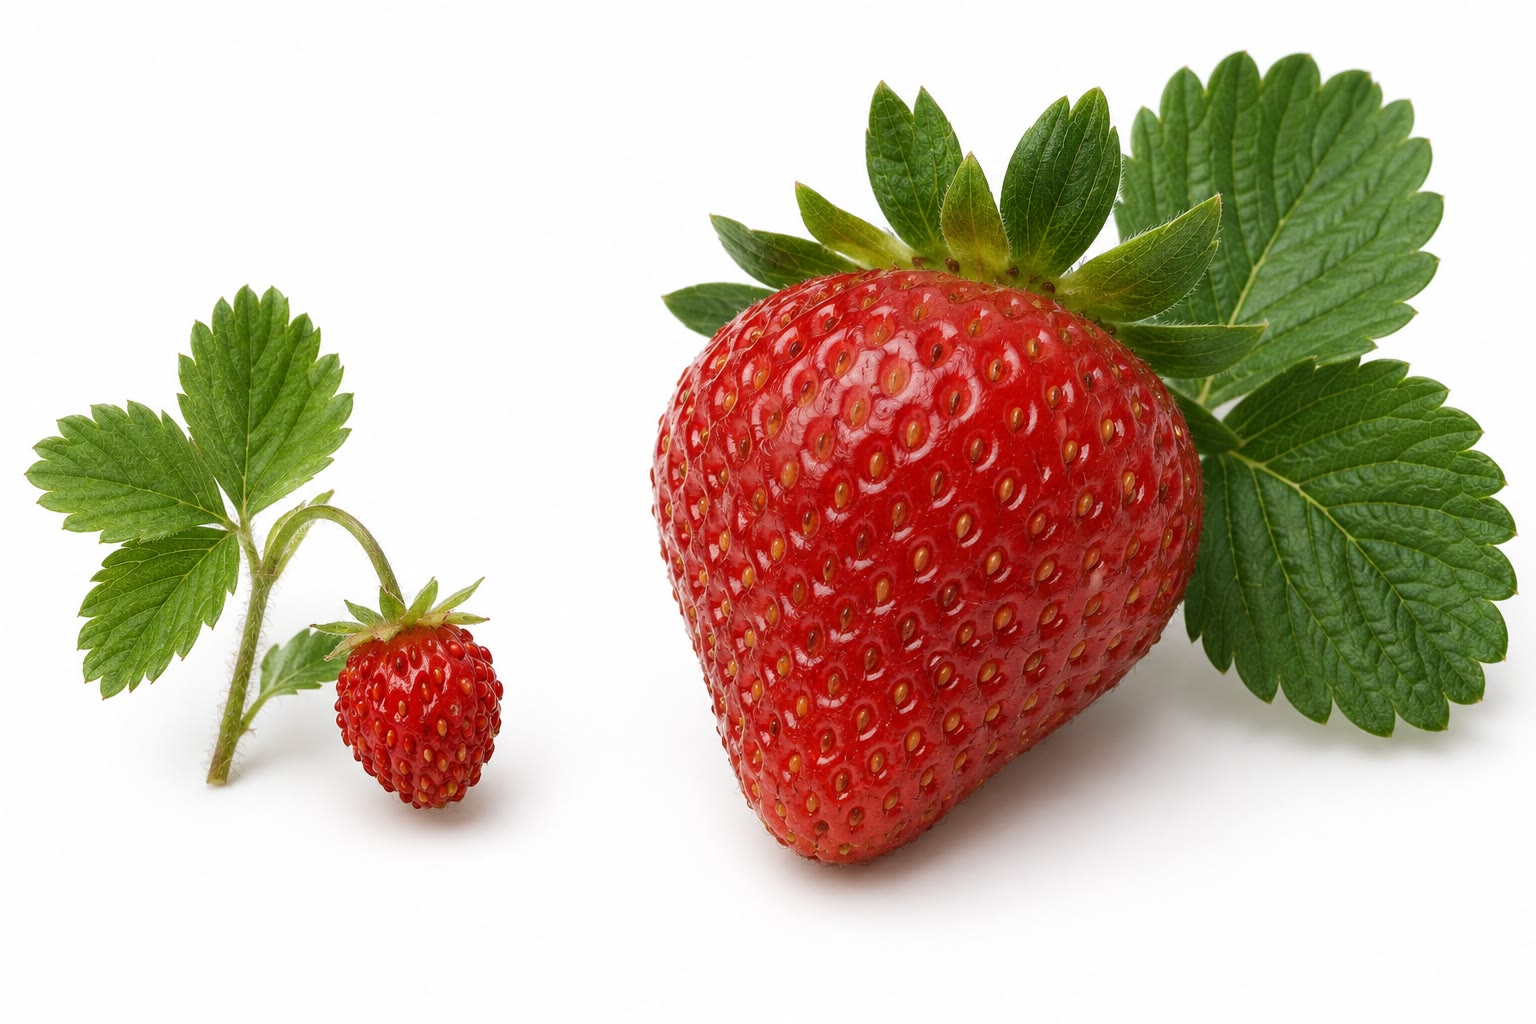
\includegraphics[width=0.55\linewidth]{images/book4/ai/b4-03-polyploid-strawberries.jpg}

{\small Arbei diploid liar dan arbei budi daya yang oktoploid: si
\omterm{def:b2:genome-diversification:polyploidy}{poliploid}, dengan DNA empat kali lipat di dalam tiap selnya, adalah
tumbuhan yang lebih besar dengan buah yang lebih besar.}
\end{omfigure}

\section{Keacakan dan laju}

\begin{proposition}[Mutasi acak terhadap kebutuhan]\label{prop:b2:genome-diversification:random}
\index{mutasi!keacakannya}
\omterm{thm:b2:genome-diversification:luria}{Uji fluktuasi} dan pelempengan replika menunjukkan bahwa sebuah \omterm{def:b2:genome-diversification:mutation}{mutasi}
yang berguna di lingkungan baru muncul pada laju yang sama entah
lingkungan itu hadir atau tidak: lingkungannya menyeleksi di antara
\omterm{def:b2:genome-diversification:mutation}{mutasi}, ia tidak memanggilnya keluar. \omterm{def:b2:genome-diversification:mutation}{Mutasi} tidak acak dalam
setiap arti --- transisi lebih banyak daripada transversi, dinukleotida
CpG bermutasi sepuluh kali lebih cepat daripada tapak lain (sitosina
termetilasinya terdeaminasi menjadi timina, yang tidak dikenali
perbaikannya sebagai asing), beberapa daerah menjadi titik panas, dan
tekanan dapat menaikkan laju keseluruhannya --- tetapi ia buta terhadap
akibatnya. \omterm{thm:b2:genome-diversification:rate}{Laju mutasinya} sendiri adalah sifat terwariskan, dan
seleksi menalanya: terlalu tinggi, tiap generasinya mewarisi perubahan
yang merugikan; terlalu rendah, populasinya tidak sanggup mengikuti
dunia yang berubah. Galur mutator menang sebentar di rumah sakit dan
kalah dalam jangka panjang, dan laju $10^{-9}$ tiap basa yang
disepakati sebagian besar sel adalah sebuah kompromi antara ongkos
kekeliruan dan ongkos pengoreksian.
\end{proposition}

\section{Latihan}

\begin{exercise}[$\star$]\label{exo:b2:genome-diversification:1}
Golongkanlah tiap perubahan pada kodon GAA (glutamat): GAG; GTA; TAA;
insersi sebuah C sesudah basa pertamanya. Mana yang transisi dan mana
yang transversi?
\end{exercise}

\begin{exercise}[$\star$]\label{exo:b2:genome-diversification:2}
Dengan $u = \qty{5e-10}{}$ tiap pasangan basa tiap replikasi dan $G =
\qty{4.6e6}{}$, berapa \omterm{def:b2:genome-diversification:mutation}{mutasi} baru yang dihasilkan satu pembelahan
\emph{E.~coli} secara rata-rata? Berapa banyak tiap generasi di dalam
biakan berisi $10^{9}$ sel?
\end{exercise}

\begin{exercise}[$\star$]\label{exo:b2:genome-diversification:3}
Sebutkan ketiga jalan \omterm{def:b2:genome-diversification:hgt}{pemindahan gen mendatar} lalu katakan, untuk
masing-masing, apa yang dibutuhkannya (sentuhan, sebuah virus, DNA
bebas) dan apa yang lazimnya dipindahkannya.
\end{exercise}

\begin{exercise}[$\star$]\label{exo:b2:genome-diversification:4}
Bedakanlah autopoliploidi dari alopoliploidi, dengan sebuah contoh
masing-masing, lalu jelaskan mengapa hibrid diploid dua spesies
biasanya mandul.
\end{exercise}

\begin{exercise}[$\star\star$]\label{exo:b2:genome-diversification:5}
Garis nutfah manusia menimbun $u = \qty{1.2e-8}{}$ \omterm{def:b2:genome-diversification:mutation}{mutasi} tiap
pasangan basa tiap generasi pada genom haploid berisi \qty{3.2e9}{}
pasangan basa. Berapa \omterm{def:b2:genome-diversification:mutation}{mutasi} baru yang diusung seorang anak? Kalau
\qty{1.5}{\%} genomnya menyandikan protein dan \qty{70}{\%} substitusi
penyandi mengubah sebuah asam amino, berapa perubahan asam amino baru
yang diusung anak itu?
\end{exercise}

\begin{exercise}[$\star\star$]\label{exo:b2:genome-diversification:6}
Sebuah biakan tumbuh dari $10^{3}$ menjadi $10^{9}$ sel; sebuah \omterm{def:b2:genome-diversification:mutation}{mutasi}
tertentu terjadi pada $m = \qty{2e-8}{}$ tiap pembelahan. Hitunglah
harapan cacah peristiwa \omterm{def:b2:genome-diversification:mutation}{mutasi} dan cacah sel mutannya. Mengapa bagian
biakan yang tak bermutan tidak berguna di sini untuk mengukur $m$, dan
ukuran biakan berapa yang akan membuatnya berguna?
\end{exercise}

\begin{exercise}[$\star\star$]\label{exo:b2:genome-diversification:7}
Sitosina terdeaminasi menjadi urasil; 5-metilsitosina terdeaminasi
menjadi timina. Jelaskan mengapa yang pertama diperbaiki secara
berdaya guna dan yang kedua tidak, lalu simpulkan mengapa tapak CpG
(tempat sitosinanya termetilasi) menjadi titik panas \omterm{def:b2:genome-diversification:mutation}{mutasi} dan lebih
langka di dalam genomnya daripada ramalan peluang semata.
\end{exercise}

\begin{exercise}[$\star\star$]\label{exo:b2:genome-diversification:8}
Dalam sebuah percobaan perkawinan terputus, empat gen memasuki
penerimanya pada 8, 17, 25, dan \qty{40}{min}; seluruh kromosomnya
(\qty{4.6}{Mb}) akan memakan \qty{100}{min}. Ubahlah waktunya menjadi
kedudukan dalam kilobasa lalu hitunglah jarak antargen berurutan.
\end{exercise}

\begin{exercise}[$\star\star$]\label{exo:b2:genome-diversification:9}
Gambarkanlah pemasangan dan pindah silang yang mengubah dua kromosom
yang masing-masing bergen $\alpha$-globin berderet dua menjadi satu
kromosom bergen tiga dan satu kromosom bergen satu. Seseorang mewarisi
kromosom bergen satu dari tiap tetuanya: berapa gen $\alpha$ yang
dimilikinya, dan apa yang diharapkan dari hemoglobinnya?
\end{exercise}

\begin{exercise}[$\star\star\star$]\label{exo:b2:genome-diversification:10}
Gandum roti adalah AABBDD dengan $2n = 42$. Sebutkan cacah kromosom
gametnya, cacah kromosom hibrid mandul pada tiap langkah asal mulanya,
dan cacah kromosom persilangan antara gandum roti dan gandum emer
(AABB). Jelaskan dari segi pemasangan meiosis mengapa tiap penggandaan
memulihkan kesuburannya dan mengapa si heksaploid tak dapat
disilangbalikkan dengan tetuanya.
\end{exercise}

\begin{exercise}[$\star\star\star$]\label{exo:b2:genome-diversification:11}
Di dalam populasi usus berisi $N = 10^{9}$ bakteri, sebuah \omterm{def:b2:unicellular-diversity:prokaryote}{plasmid}
kekebalan menyebar lewat konjugasi pada laju yang sebanding dengan
perjumpaan antara pengusungnya $R$ dan yang bukan pengusung $N - R$:
$\mathrm{d}R/\mathrm{d}t =
\gamma R (N - R)$ dengan $\gamma N = \qty{0.5}{h^{-1}}$. Pecahkanlah,
dimulai dari satu pengusung, lalu hitunglah waktu bagi separuh
populasinya untuk mengusung \omterm{def:b2:unicellular-diversity:prokaryote}{plasmidnya}. Apa yang terjadi kalau
antibiotiknya lalu ditarik dan \omterm{def:b2:unicellular-diversity:prokaryote}{plasmidnya} memakan \qty{5}{\%} laju
pertumbuhan inangnya?
\end{exercise}

\begin{exercise}[$\star\star\star$]\label{exo:b2:genome-diversification:12}
``\omterm{def:b2:genome-diversification:mutation}{Mutasi} bersifat acak; evolusi tidak.'' Bahaslah, dengan memakai
\omterm{thm:b2:genome-diversification:luria}{uji fluktuasi}, pelempengan replika, dan kenyataan bahwa \omterm{thm:b2:genome-diversification:rate}{laju
mutasinya} sendiri berada di bawah seleksi.
\end{exercise}

\section{Soal: Sebuah Uji Fluktuasi}

\begin{problem}[{Soal akhir pekan --- sebuah uji fluktuasi dijalankan
dan dianalisis, laju mutasi sebuah galur ditarik darinya lalu diskalakan
ke genom dan populasinya, penyebaran sebuah plasmid kekebalan dimodelkan,
dan ongkos seorang mutator ditimbang, berakhir pada laju mutasi galur
itu tiap basa dan waktu plasmidnya mengambil alih}]
\label{pb:b2:genome-diversification:1}
Dua puluh biakan \emph{E.~coli} masing-masing dimulai dari \num{100}
sel dalam \qty{0.2}{mL} lalu ditumbuhkan sampai $N = \qty{2e8}{}$ sel;
masing-masing kemudian disebarkan pada sebuah lempeng berbakteriofag,
dan koloni yang kebal dicacah: 0, 0, 0, 1, 0, 0, 3, 0, 0, 1, 0, 0, 0,
0, 107, 0, 2, 0, 0, 5. Sejajar dengan itu, dua puluh contoh
\qty{0.2}{mL} diambil dari satu biakan besar pada kerapatan yang sama
lalu dilempengkan dengan cara yang sama: 14, 15, 13, 21, 15, 14, 26,
16, 20, 13, 17, 12, 18, 14, 16, 19, 15, 13, 17, 16. Genomnya:
\qty{4.6e6}{} pasangan basa, \qty{88}{\%} penyandi. Kekebalan terhadap
fagnya dapat muncul lewat salah satu dari \num{20} perubahan basa
tunggal yang berbeda pada satu gen reseptor.

\medskip
\noindent\textbf{Bagian I --- Ujinya.}
\begin{enumerate}
  \item Hitunglah purata dan ragam kedua puluh biakan yang saling
        bebas itu.
  \item Hitunglah purata dan ragam kedua puluh contohnya.
  \item Bagi sebaran Poisson, ragamnya sama dengan puratanya.
        Perangkat mana yang Poisson, dan apa yang dikatakan sebaran
        tiap perangkatnya tentang \emph{kapan} \omterm{def:b2:genome-diversification:mutation}{mutasinya} terjadi?
  \item Jelaskan cacah 107 itu.
  \item Berapa banyak biakan bebas itu yang tidak memuat mutan?
        Pakailah $p_0 = e^{-m(N - N_0)}$ untuk menaksir $m$, yaitu \omterm{thm:b2:genome-diversification:rate}{laju
        mutasi} menuju kekebalan tiap pembelahan sel.
  \item Hitunglah harapan cacah sel mutan tiap biakannya dari
        $mN\ln(N/N_0)$ lalu bandingkan dengan purata amatannya.
  \item Mengapa contoh dari biakan tunggal itu tidak akan berguna untuk
        menaksir $m$ dengan cara $p_0$?
\end{enumerate}

\medskip
\noindent\textbf{Bagian II --- Menskalakannya ke genom.}
\begin{enumerate}[resume]
  \item Simpulkan \omterm{thm:b2:genome-diversification:rate}{laju mutasi} $u$ tiap pasangan basa tiap replikasi
        dari $m$ dan cacah perubahan yang memberikan kekebalan.
  \item Hitunglah purata cacah \omterm{def:b2:genome-diversification:mutation}{mutasi} baru tiap genom tiap
        replikasi, yaitu $U$.
  \item Sebuah biakan satu liter pada $10^{9}$ sel tiap mililiter
        berlipat dua sekali. Berapa \omterm{def:b2:genome-diversification:mutation}{mutasi} baru yang muncul di dalam
        populasinya?
  \item Berapa banyak perubahan basa tunggal yang berbeda yang mungkin
        pada genom ini? Secara rata-rata, berapa kali masing-masing
        muncul dalam satu kali pelipatduaan itu?
  \item Jelaskan mengapa, pada populasi semacam itu, kekebalan terhadap
        antibiotik tunggal mana pun yang dapat dikalahkan satu \omterm{def:b2:genome-diversification:mutation}{mutasi}
        pada dasarnya dijamin hadir.
  \item Jelaskan mengapa menggabungkan dua antibiotik yang menuntut dua
        \omterm{def:b2:genome-diversification:mutation}{mutasi} yang saling bebas mengubah hal ini, dengan sebuah angka.
\end{enumerate}

\medskip
\noindent\textbf{Bagian III --- Sebuah \omterm{def:b2:unicellular-diversity:prokaryote}{plasmid} menyebar.}
Di dalam sebuah usus berisi $N = 10^{9}$ sel, satu sel memperoleh
sebuah \omterm{def:b2:unicellular-diversity:prokaryote}{plasmid} kekebalan konjugatif. Pengusungnya $R$ memindahkannya
pada sentuhan: $\mathrm{d}R/\mathrm{d}t = \gamma R(N - R)$, dengan $\gamma N =
\qty{0.5}{h^{-1}}$.
\begin{enumerate}[resume]
  \item Tunjukkan bahwa $R(t) = N/\bigl(1 + (N - 1)e^{-\gamma N t}\bigr)$
        memenuhi persamaannya dengan $R(0) = 1$.
  \item Hitunglah waktu ketika separuh selnya mengusung \omterm{def:b2:unicellular-diversity:prokaryote}{plasmidnya}.
  \item Hitunglah waktu ketika \qty{99}{\%} selnya mengusungnya.
  \item Berapa peristiwa konjugasi tiap jam yang berlangsung pada saat
        separuh selnya menjadi pengusung?
  \item Bandingkan dengan waktu bagi sebuah \emph{mutan} kebal untuk
        mencapai separuh populasinya dengan tumbuh \qty{10}{\%} lebih
        cepat daripada sisanya di bawah antibiotiknya (\omterm{def:b2:unicellular-diversity:division}{waktu generasi}
        \qty{1}{h} bagi sel yang peka): dimulai dari satu sel, berapa
        lama waktunya?
  \item Simpulkan mengapa kekebalan terutama menyebar lewat pemindahan
        dan bukan lewat pewarisan.
\end{enumerate}

\medskip
\noindent\textbf{Bagian IV --- Seorang mutator.}
Sebuah galur yang tidak memiliki perbaikan salah pasang bermutasi
\num{100} kali lebih cepat. Andaikan \qty{30}{\%} \omterm{def:b2:genome-diversification:mutation}{mutasi} di
dalam urutan penyandi bersifat merugikan.
\begin{enumerate}[resume]
  \item Hitunglah $U$-nya dan purata cacah \omterm{def:b2:genome-diversification:mutation}{mutasi} merugikan tiap
        sel tiap generasi.
  \item Sesudah \num{200} generasi, berapa bagian keturunan sebuah
        garis keturunan yang sama sekali tidak mengusung \omterm{def:b2:genome-diversification:mutation}{mutasi}
        merugikan (Poisson)?
  \item Hitunglah nilai yang sama bagi tipe liarnya.
  \item Pada \omterm{thm:b2:genome-diversification:luria}{uji fluktuasi} di atas, purata cacah berapa yang akan
        diberikan mutatornya, dan berapa bagian biakan yang tidak
        bermutan?
  \item Jelaskan dalam dua kalimat mengapa mutator ditemukan di antara
        isolat rumah sakit dan langka di alam.
  \item Nyatakan hasilnya: $m$, $u$, dan $U$ bagi galurnya, serta waktu
        bagi \omterm{def:b2:unicellular-diversity:prokaryote}{plasmidnya} mencapai separuh dan \qty{99}{\%} ususnya.
\end{enumerate}
\end{problem}
